\documentclass[10pt,a4paper,twocolumn,twoside]{article}
\usepackage[utf8]{inputenc}
\usepackage[catalan]{babel}
\usepackage{multicol}
\usepackage{graphicx}
\usepackage{fancyhdr}
\usepackage{times}
\usepackage{titlesec}
\usepackage{multirow}
\usepackage[top=2.5cm, bottom=1.3cm, left=1.2cm, right=1.2cm]{geometry}
\usepackage[figurename=Fig.,tablename=Taula,font={small,sf}]{caption}
%\usepackage[font={small,sf}]{caption}

\usepackage{enumitem}
\setlist[itemize]{noitemsep}
\setlist[enumerate]{noitemsep}

\let\OLDthebibliography\thebibliography
\renewcommand\thebibliography[1]{
  \OLDthebibliography{#1}
  \setlength{\parskip}{0pt}
  \setlength{\itemsep}{0pt plus 0.3ex}
}

\pagestyle{fancy}
\fancyhf{}
\fancyhead[LO]{\textsf{\small $\mu$Projecte VC(GEI)-PSIV(GED), Escola d’Enginyeria (EE), Universitat Autònoma de Barcelona (UAB)}}
\fancyhead[RE]{\textsf{\small $\mu$Projecte VC(GEI)-PSIV(GED), Escola d’Enginyeria (EE), Universitat Autònoma de Barcelona (UAB)}}
\renewcommand{\headrulewidth}{0pt}

\titleformat*{\section}{\large\sffamily\scshape\bfseries}
\titleformat*{\subsection}{\normalsize\sffamily\bfseries}
\titleformat*{\subsubsection}{\normalsize\sffamily\slshape}

\begin{document}

{\sffamily
% Titol
\noindent\textbf{\LARGE Títol explicatiu i relatiu al contingut del treball}
% autors
\begin{center}
María Dolores Flores Ruiz, Manuel Ortega Juárez
\end{center}

\bigskip
\bigskip

\noindent 
\textbf{Abstract}--- Lorem ipsum dolor sit amet, consectetur adipiscing elit. In auctor est et lacus luctus eleifend. Duis at tincidunt nibh. Nam sed elementum lorem, eu pretium magna. Vestibulum justo urna, imperdiet eget tristique ut, pellentesque vel turp-is. Vivamus et risus tempor, fringilla libero in, semper arcu. Praesent blandit libero vitae rutrum tincidunt. Fusce id justo quis mauris accumsan pellentesque et in massa. Nulla ut eleifend ante. Nunc pretium justo a nibh tincidunt tempus. Fusce auctor tortor nec turpis commodo, vitae posuere nulla mollis. Maecenas non placerat metus. Mauris dolor libero, laoreet quis leo vitae, dignissim lobortis enim. Curabitur in magna nibh. Aenean vel dui eros. Morbi maximus in turpis vitae fermentum.

Duis interdum nisi id sem dictum rhoncus. Duis vitae ante tincidunt, tempor diam quis, tincidunt lorem. Etiam sit amet nisi tempus sapien auctor vestibulum ac eu purus. Curabi-tur a suscipit urna, sit amet facilisis erat. Morbi iaculis ves-tibulum tortor, quis varius justo mollis ut. Pellentesque plac-erat felis pretium, maximus ex quis, rutrum nisi. Sed quis imperdiet nunc. Donec euismod ipsum sed urna semper posuere. Nunc id gravida enim. Suspendisse tortor lectus, tempus tincidunt tellus at, mattis tincidunt tortor. Morbi fini-bus ultrices bibendum. Morbi ac ipsum eu erat consectetur convallis at. 

\bigskip

\noindent 
\textbf{Keywords}---Image classification, noisy web data, CNNs, ubiquitous reweighting.
}
\bigskip

{\vrule depth 0pt height 0.5pt width 3cm\hspace{7.5pt}%
\raisebox{-3.5pt}{\fontfamily{pzd}\fontencoding{U}\fontseries{m}\fontshape{n}\fontsize{11}{12}\selectfont\char70}%
\hspace{7.5pt}\vrule depth 0pt height 0.5pt width 3cm\relax}

\bigskip


\section{Introducció}

Aquest document és una adaptació dels articles de la IEEE i del TFG i assumeix la utilització de \LaTeX \cite{latex}. 

Teniu ja l'estructura de punts a omplir. Podeu fer subseccions en cadascun dels punts. Podeu afegir punts extres si ho considereu necessari. La mida final no pot sobrepassar les quatre pàgines i podeu redactar-lo en català, castellà o anglès. Respecteu el format el màxim possible per unificar tots els treballs.

%\begin{itemize} %equivalències aproximades en word
%\item	text abstract: Arial 9
%\item	text general: Times New Roman 10
%\item	títol: Arial 16, negreta
%\item	títols de seccions: Arial 12, negreta
%\item	títols de subseccions: Arial 10, negreta
%\item	Figures: Fig. \#. Arial 9
%\item	Taules: Taula \#. Tabla \#. o Table \#. Arial 9
%\item	text referències: Times New Roman 9
%\item	Justificació completa a tot el document
%\end{itemize}

Podeu alterar les seccions, però amb aquesta base ja es pot explicar tot el que se sol explicar en un petit article. 

El títol ha de ser clar sobre el que trobarem en l’article, millor si no hi ha clickbait. A la part de la introducció, s'ha d’explicar el context del projecte les possibles motivacions i els objectius que es volen aconseguir. A la part de l’estat de l’art heu de fer una recopilació de com s’ha abordat aquest projecte per altra gent, fent més èmfasi en les tècniques més actuals. En la secció de proposta (que podria ser material i mètode o desenvolupament) podeu desplegar les vostres idees de com resoldre el projecte i quines dades en fareu servir i d’on sortiran. Han de ser dades que existeixen no propostes de dades. La secció d’experiment, resultats i anàlisi ha d’enumerar les proves realitzades, els resultats aconseguits i una petita discussió local d’aquests. La part de conclusió és una recapitulació i destil·lació del que hem après amb el desenvolupament del projecte. A les referències heu de citar totes aquelles fonts bibliogràfiques que us hagin aportat pistes i documentació per fer el projecte. I finalment, un cop acabat heu de fer l’abstract que és un resum de tot: de la intro, l’objectiu principal, l’estat de l’art, la vostra proposta i els principals resultats aconseguits. Pot haver-hi spoilers a l’abstract en aquest tipus d’articles. 

Aquest document l’haureu de lliurar un parell de vegades: (i) una primera vegada, però no complert, amb la intro amb els objectius, l'estat de l'art, la proposta amb el tipus i fonts de dades i les referències; (ii) l'entrega final, amb no més de quatre pàgines amb totes les seccions esmentades.

Per aquest primer lliurament els punts a tenir en compte són:

\begin{itemize}
\item	Llista treballs previs relacionats que tens prevists revisar per desenvolupar el teu sistema.
\item	Descriu com construiràs una base d’imatges/vídeos per desenvolupar la teva proposta.
\item	Estructura el flux de procés que conformarà el teu sistema de visió.
\item	Recull tècniques amb potencial per a ser aplicades als diferents passos del flux proposat.
\item	Detalla com penses mesurar el rendiment del teu sistema.
\end{itemize}

La resta del document no té informació rellevant llevat de com mostrar figures (vegeu Fig. \ref{f:vistageneral} i Fig \ref{f:detall}), en alguns casos es poden fer servir figures que omplin les dues columnes; taules (vegeu Taula \ref{t:raonstrigonometriques}), equació com la identitat d’Euler \ref{eq:igualtatdeuler}, i referències\cite{Russakovskyet2015} ,\cite{Krizhevsky2012} ,
\cite{Simonyan2014} ,\cite{Szegedyet2015}. També l’estructura i la divisió de les diferents seccions.



\begin{equation}
 e^{i\pi}+1=0 \quad,
\label{eq:igualtatdeuler}
\end{equation}

\section{Estat de l'art}

\subsection{Exemple de subsecció}

Lorem ipsum dolor sit amet, consectetur adipiscing elit. Curabitur quis fermentum orci. Aliquam sodales varius blandit. Vestibulum congue tortor a fringilla venenatis. Nam magna ex, fringilla eu porta facilisis, consequat quis orci. Vivamus ut mattis metus. Interdum et malesuada fames ac ante ipsum primis in faucibus. Maecenas a orci at nibh so-dales condimentum. Orci varius natoque penatibus et mag-nis dis parturient montes, nascetur ridiculus mus. 

Mauris sodales, ex nec egestas suscipit, augue ante vehi-cula dolor, sed mattis erat elit a neque. Sed pulvinar, metus ut vulputate posuere, tellus erat hendrerit erat, vitae fringilla neque tellus at risus. Ut dictum lacinia pharetra. Praesent nec volutpat sapien. Maecenas convallis elit at justo ul-lamcorper scelerisque. Curabitur elementum arcu nec mau-ris pulvinar vulputate. Quisque lacus turpis, porta nec auctor a, fringilla vel ante. Vivamus sit amet lectus mattis, faucibus metus rhoncus, sodales quam. Aliquam eu fermentum justo, a porttitor dolor. Etiam ac mattis metus. Proin eget massa vel velit tristique accumsan non eu eros. Cras ultricies ali-quam ante in facilisis. Aliquam ante magna, vehicula nec diam ac, lacinia accumsan ante. Cras hendrerit vehicula ante, et varius diam congue sit amet. Class aptent taciti sociosqu ad litora torquent per conubia nostra, per inceptos himenaeos. Nullam id iaculis lectus. 


\subsection{Exemple de subsecció}

Suspendisse potenti. Maecenas lacinia est a mauris fau-cibus, vitae eleifend ante ornare. In hac habitasse platea dictumst. Etiam accumsan ligula vel mauris sagittis, quis mollis felis tincidunt. In semper sem a mi malesuada, sit amet venenatis magna sollicitudin. Class aptent taciti soci-osqu ad litora torquent per conubia nostra, per inceptos himenaeos. Proin id enim ut odio ultrices condimentum porta eget enim. Nulla nec metus pretium, sollicitudin lectus pretium, lobortis enim. Nunc consectetur eget enim eu ia-culis. Aenean a purus porttitor, posuere orci in, consequat lorem. Nam lobortis tristique lacus feugiat dapibus. Etiam gravida blandit volutpat. 

Sed aliquam lectus at dolor ultrices rhoncus. Pellentesque tincidunt urna dui, eget accumsan sem pharetra id. Etiam vel venenatis tortor. Nullam ornare massa eu velit mollis vulputate. In ultricies urna non arcu sollicitudin vestibulum. Praesent semper at lacus mattis hendrerit. Vestibulum pel-lentesque ut ex quis mollis. Fusce porttitor vitae odio preti-um ornare. Praesent varius nec tortor at consectetur. Nam malesuada diam id velit elementum efficitur. Fusce ali-quam, magna amet rhoncus sollicitudin, risus tellus ultrices eros, ac venenatis tortor velit non arcu. Sed et massa iaculis, viverra erat ut, rutrum justo. Suspendisse semper, metus sed bibendum ultricies, elit felis varius mauris, in tincidunt velit odio sit amet elit. Donec vel metus eu libero vehicula pharetra nec at purus. 

Fusce non finibus odio. Lorem ipsum dolor sit amet, con-sectetur adipiscing elit. Fusce ultrices euismod ipsum in malesuada. Cras consectetur sed ipsum vel placerat. In nec turpis eu orci dictum tincidunt in feugiat dolor. Donec mi nibh, aliquam eget vestibulum ac, consequat condimentum nulla. Ut lectus erat, ultrices non viverra nec, tincidunt ut velit. Proin elementum odio rhoncus nulla ultricies, id ac-cumsan tortor accumsan. 


\section{Proposta}

Donec in lorem eget nulla posuere auctor. Duis tempor tincidunt leo, eget vestibulum orci rutrum vitae. Nam non metus feugiat, malesuada nibh ac, bibendum sem. Sus-pendisse pretium, enim id gravida mattis, enim sapien ele-mentum erat, vel varius ligula erat sed sem. Quisque nec convallis ligula. Duis nec ante interdum, varius nibh sit amet, volutpat turpis. Nulla dignissim egestas augue, euismod laoreet nisi efficitur varius. Donec eu enim viverra, maximus ipsum sed, porta ipsum. Donec massa lectus, suscipit et sapien ac, ornare feugiat ipsum. Nulla vehicula metus tellus, id viverra nisi sodales eu. Vivamus tempor augue ac eros feugiat facilisis. Donec lacus massa, aliquet et finibus vitae, imperdiet id ligula. Suspendisse convallis congue dui, at pulvinar sapien commodo ut. Interdum et malesuada fames ac ante ipsum primis in faucibus. Proin laoreet maximus lacus, sed lobortis quam tincidunt a. Suspendisse potenti. 

Quisque et odio elit. Cras bibendum felis vitae neque tin-cidunt ornare. Quisque viverra sodales ullamcorper. Orci varius natoque penatibus et magnis dis parturient montes, nascetur ridiculus mus. Maecenas molestie lacinia nunc, non tempus ligula placerat ac. Proin eget nibh eget lorem sodales viverra at luctus lectus. Etiam mollis ante ac eros mollis convallis. Pellentesque dignissim blandit nisl, ac accumsan risus congue id. Class aptent taciti sociosqu ad litora tor-quent per conubia nostra, per inceptos himenaeos. Aliquam nibh odio, ullamcorper quis iaculis et, rutrum ac elit. Morbi posuere tempus tempus. Nullam arcu diam, tincidunt phare-tra enim eu, fringilla accumsan nisi. Nullam vitae tempor tortor. Mauris vel ipsum sit amet ante venenatis ultrices et ut odio. 

Nunc dictum ipsum quis egestas scelerisque. Vestibulum rutrum tempor posuere. Praesent varius libero odio, ac bibe-ndum arcu tempus quis. Pellentesque habitant morbi tristi-que senectus et netus et malesuada fames ac turpis egestas. Sed eget ex risus. Integer metus velit, viverra ac fringilla sit amet, laoreet eget lacus. Nulla rutrum mollis elit et maximus. Nulla sed aliquet elit. Sed libero justo, porta ut vulputate eget, suscipit faucibus sem. Sed at quam ut justo vestibulum vehicula non sed ligula. Nulla facilisi. Curabitur pulvinar, dolor amet ultrices porttitor, odio nisl tincidunt magna, cras lobortis metus tristique erat placerat, sed dapibus elit tellus vel mauris.

Ut interdum risus a diam mollis iaculis. Nulla facilisi. Donec consequat feugiat leo vitae interdum. Aliquam eges-tas dolor a enim vehicula sollicitudin. Nam et tellus augue. Aenean luctus ac ipsum a condimentum. Donec quam nunc, bibendum sed ornare et, sollicitudin eget nulla. Aenean viverra ipsum interdum, ultricies ante volutpat, tincidunt est. Suspendisse tempor orci ut ullamcorper mollis. Duis sceler-isque sapien bibendum neque eleifend, in ullamcorper ante lobortis. Vivamus quis eleifend metus. Praesent varius nec tortor at consectetur. Aliquam convallis velit vel nulla rhon-cus, tempor blandit velit dictum. Mauris quis felis a elit con-sequat tempor sit amet a odio. In sit amet augue id nisl ultri-cies fringilla. 

Nam facilisis fringilla venenatis. Aliquam turpis lacus, euismod ac lorem nec, rutrum congue sem. Donec et conse-quat turpis. Etiam a mauris lorem. Duis pharetra rutrum magna, a placerat diam blandit nec. Donec justo nibh, ul-lamcorper sed dictum non, accumsan id est. Praesent nec placerat mauris. Sed consequat risus risus. Aliquam in eros quis neque tempus dictum vitae ut est. Nam tempus sed turpis nec dignissim. Proin id enim ut odio ultrices condimen-tum porta eget enim. Donec vestibulum lorem in mattis luctus. Donec a leo quis nibh accumsan iaculis. Duis fauci-bus mi elit. Nulla neque ex, tempor vel dolor id, ultricies aliquet nulla.

 
\section{Experiments, resultats i anàlisi}

Curabitur tempor a augue et vestibulum. Mauris fermen-tum lorem lectus, vitae vestibulum leo faucibus quis. Mauris non leo ligula. Donec ac egestas orci. Pellentesque rhoncus leo porta augue dictum tristique. Nam ullamcorper egestas sem, a posuere dui placerat nec. Vivamus eget dictum sem. Aliquam bibendum dui auctor tellus viverra, eu molestie leo consectetur. Duis tristique elit velit, aliquam posuere risus condimentum ac. 

Ut hendrerit porttitor metus, nec elementum sem. Proin quis purus elit. Vivamus eu aliquam nulla. Duis consectetur neque cursus nibh fermentum, eget facilisis sapien fringilla. In luctus massa vitae blandit pharetra. Suspendisse et sem nunc. Integer rutrum tellus id volutpat pellentesque. Mauris vulputate quam sit amet mollis luctus. Nam facilisis fringilla venenatis. Aliquam turpis lacus, euismod ac lorem nec, rut-rum congue sem. Donec et consequat turpis. Etiam a mauris lorem. Duis pharetra rutrum magna, a placerat diam blandit nec. Proin turpis nunc, ultricies vel rutrum quis, sollicitudin eget leo. Nullam at semper ex. Pellentesque a purus lacus. Vestibulum porttitor bibendum neque. 

\subsection{Exemple de subsecció}


Sed in leo rhoncus, gravida elit vel, tristique quam. Nu-llam auctor mi in tortor mollis ullamcorper. Duis mattis nisl purus. Maecenas posuere libero sem, a vulputate erat elei-fend eu. Proin a iaculis enim. Suspendisse potenti. Vestibu-lum egestas sed erat ac porttitor. Vestibulum a est risus. Sus-pendisse potenti. Donec eleifend dui erat, vel blandit nisl dignissim sit amet.Quisque et odio elit. Cras bibendum felis vitae neque tin-cidunt ornare. 

Nunc dictum ipsum quis egestas scelerisque. Vestibulum rutrum tempor posuere. Praesent varius libero odio, ac bibe-ndum arcu tempus quis. Pellentesque habitant morbi tristi-que senectus et netus et malesuada fames ac turpis egestas. Sed eget ex risus. Integer metus velit, viverra ac fringilla sit amet, laoreet eget lacus. Nulla rutrum mollis elit et maximus. Nulla sed aliquet elit. Sed libero justo, porta ut vulputate eget, suscipit faucibus sem. Sed at quam ut justo vestibulum vehicula non sed ligula. Nulla facilisi. Curabitur pulvinar, dolor amet ultrices porttitor, odio nisl tincidunt magna, cras lobortis metus tristique erat placerat, sed dapibus elit tellus vel mauris.

Integer maximus, diam eu tristique tincidunt, tellus sem sagittis urna, ac viverra nisi nibh nec lectus. Morbi mollis tincidunt ligula, in vestibulum lectus condimentum eu. Cras nec porttitor nibh. Fusce bibendum eu nunc nec eleifend. Morbi id nulla accumsan nisi suscipit tempus. Donec mollis sem enim. Praesent hendrerit dignissim tellus nec imperdiet. 

Pellentesque ex dolor, ullamcorper et tempus ac, feugiat vel ligula. Cras ut sagittis nisi. Nunc mauris turpis, dignissim ut lorem vitae, suscipit vulputate mi. Curabitur at elit neque. Nam ornare vel turpis tempus eleifend. Morbi faucibus risus eros, sit amet congue lectus tristique a. Aenean ut egestas ex. Vivamus consequat eu odio sit amet mattis. Nullam pretium sodales eleifend. Fusce fermentum risus ac nisi interdum, ornare vestibulum metus laoreet. Cras finibus nisi eu biben-dum viverra. Maecenas vel nulla sed nibh suscipit iaculis id imperdiet elit. Mauris a enim enim. Etiam vestibulum odio ac elit iaculis sollicitudin. In mollis in erat ut malesuada. 

Donec pharetra mollis nisi, sit amet lobortis ligula. Nunc aliquam ornare diam, ac faucibus est pellentesque ut. Mae-cenas eget bibendum urna. 

\begin{table}[!h]
\centering
\begin{tabular}{lccccc}
 x & sin(x) &	cos(x)& tan(x) &  sec(x) & cosec(x)\\
\hline
30$^\circ$ & 0.5000 & 0.8660 & 0.5774 & 1.1547 & 2.0000\\
45$^\circ$ & 0.7071 & 0.7071 & 1.0000 & 1.4142 & 1.4142\\
60$^\circ$ & 0.8660 & 0.5000 & 1.7321 & 2.0000 & 1.1547\\
\hline
\end{tabular}
\caption{ Raons trigonomètriques per diferents valors d’angles.}
\label{t:raonstrigonometriques}
\end{table}

Pellentesque congue lorem ut lacus vehicula ultricies. Nunc ullamcorper porttitor est, vel faucibus magna viverra laoreet. Mauris nec tortor augue. Integer elementum ac nulla ut dictum. Vestibulum quis hendrerit nisl, eget suscipit mau-ris. Ut convallis aliquet tortor et pulvinar. Sed vulputate mi sed pharetra lobortis. In aliquet ex et dolor pellentesque, nec pulvinar odio iaculis. In eget ex lacus. Pellentesque dolor dui, ullamcorper eget laoreet eu, sodales nec massa. Integer maximus, diam eu tristique tincidunt, tellus sem sagittis urna, ac viverra nisi nibh nec lectus. Morbi mollis tincidunt ligula, in vestibulum lectus condimentum eu. Cras nec portti-tor nibh. Fusce bibendum eu nunc nec eleifend. Morbi id nulla accumsan nisi suscipit tempus. Donec mollis sem en-im. Praesent hendrerit dignissim tellus nec imperdiet. Proin eget nibh eget lorem sodales viverra at luctus lectus. Etiam mollis ante ac eros mollis convallis. Pellentesque dignissim blandit nisl, ac accumsan risus congue id. Class aptent taciti sociosqu ad litora tor-quent per conubia nostra, per inceptos himenaeos. 

Aliquam mi velit, sagittis et hendrerit in, hendrerit ac me-tus. Phasellus tempor est leo, non dictum metus tincidunt vel. Sed tempus rhoncus efficitur. Fusce malesuada nibh tellus, sed ullamcorper quam sodales id. Duis sapien metus, hendrerit quis lobortis vel, porta posuere dolor. Morbi in metus quis urna efficitur aliquam. Nulla rhoncus elementum sodales. Vestibulum commodo lacinia tempus. Etiam vitae euismod mi. Nam vulputate arcu a enim egestas, id pulvinar diam aliquet. Proin non vestibulum nisl.

Morbi consequat scelerisque malesuada. Mauris finibus malesuada lorem eget fermentum. Fusce vehicula ut lectus in luctus. Mauris fermentum, ipsum nec fermentum laoreet, mi nibh hendrerit augue, sed scelerisque augue nulla et justo. Curabitur neque metus, consectetur vel feugiat ac, imperdiet vitae nisl. Aliquam scelerisque id purus et tincidunt. Etiam bibendum ornare lectus, vel accumsan dui sagittis vitae. Vestibulum volutpat semper tortor, a suscipit nisi convallis id. Suspendisse potenti. Nunc nisl sapien, eleifend vitae nisl sit amet, pretium tempus massa. Pellentesque id eros ac lectus imperdiet consequat. Etiam lacus neque, bibendum vel rhoncus, tempor in est. 

% Per a fer que la figura ocupi les dues columnes utilitzeu "figure*" per comptes de "figure"
\begin{figure}[!h]
\centering
	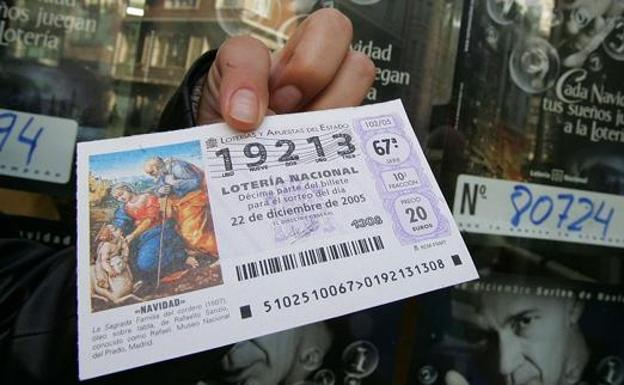
\includegraphics[width=0.4\textwidth]{figs/Fig1.jpg}
	\caption{Escena on es troba amagat el subjecte d’anàlisi. Podem veure a la dreta una andròmina amb forma de chubby robot, precursor del gènere meka i de l’aspirador roomba.}
	\label{f:vistageneral}
\end{figure}

Suspendisse blandit est vel interdum bibendum. Class ap-tent taciti sociosqu ad litora torquent per conubia nostra, per inceptos himenaeos. Aliquam erat volutpat. Ut eu leo mollis, commodo felis eu, viverra massa. Ut arcu felis, molestie fermentum neque et, ultricies fermentum purus. Nullam non ipsum odio. Suspendisse luctus, tortor at pulvinar faucibus, diam sem porttitor orci, in volutpat ligula augue sed ipsum.


Curabitur tellus turpis, fringilla ut semper vel, consectetur eget turpis. Maecenas purus nibh, dapibus quis urna quis, rutrum venenatis elit. Nulla sit amet odio vitae est hendrerit pretium vitae quis mauris. Nam interdum sed velit ac congue. Donec finibus leo vitae bibendum ornare. Nullam vestibulum lacus mi, eu gravida neque mollis eu. Nulla rhoncus elementum sodales. Vestibulum commodo lacinia tempus. Etiam vitae euismod mi. Nam vulputate arcu a enim egestas, id pulvinar diam aliquet. Proin non vestibulum nisl. Etiam imperdiet, lectus quis pellentesque lacinia, dolor ex pharetra ipsum, sit amet commodo lectus magna non est. Proin id dapibus diam. Sed semper, ligula at iaculis dignis-sim, libero ipsum dignissim elit, at ornare ipsum risus a dolor. Phasellus vitae nibh eu purus hendrerit dapibus sit amet eget diam. Donec gravida suscipit dui, nec placerat dolor congue sit amet. Donec lobortis, justo iaculis aliquam condimen-tum, felis ligula tempor nunc, ullamcorper tincidunt ante nunc vitae sapien. Aenean ante dui, condimentum non tin-cidunt a, scelerisque at quam. Praesent eu dolor sapien. Aliquam congue ornare nulla. 

Integer maximus, diam eu tristique tincidunt, tellus sem sagittis urna, ac viverra nisi nibh nec lectus. Morbi mollis tincidunt ligula, in vestibulum lectus condimentum eu. Quis-que consectetur justo a mi porta, id varius nisi posuere. Morbi tristique orci nec dolor aliquet venenatis. Integer ma-lesuada tincidunt dignissim. Cras lobortis metus tristique erat placerat, nec rutrum justo pretium. Integer faucibus aliquet commodo. Integer non quam nec lectus. Cras nec porttitor nibh. Donec gravida suscipit dui, nec placerat dolor congue sit amet. Donec lobortis, justo iaculis aliquam condimen-tum, felis ligula tempor nunc, ullamcorper tincidunt ante nunc vitae sapien. Fusce bibendum eu nunc nec eleifend. Morbi id nulla accumsan nisi suscipit tempus. Donec mollis sem enim. Praesent hendrerit dignissim tellus nec imperdiet. Phasellus vitae purus gravida, rutrum ante vel, vestibulum mauris.


\begin{figure}[!h]
\centering
	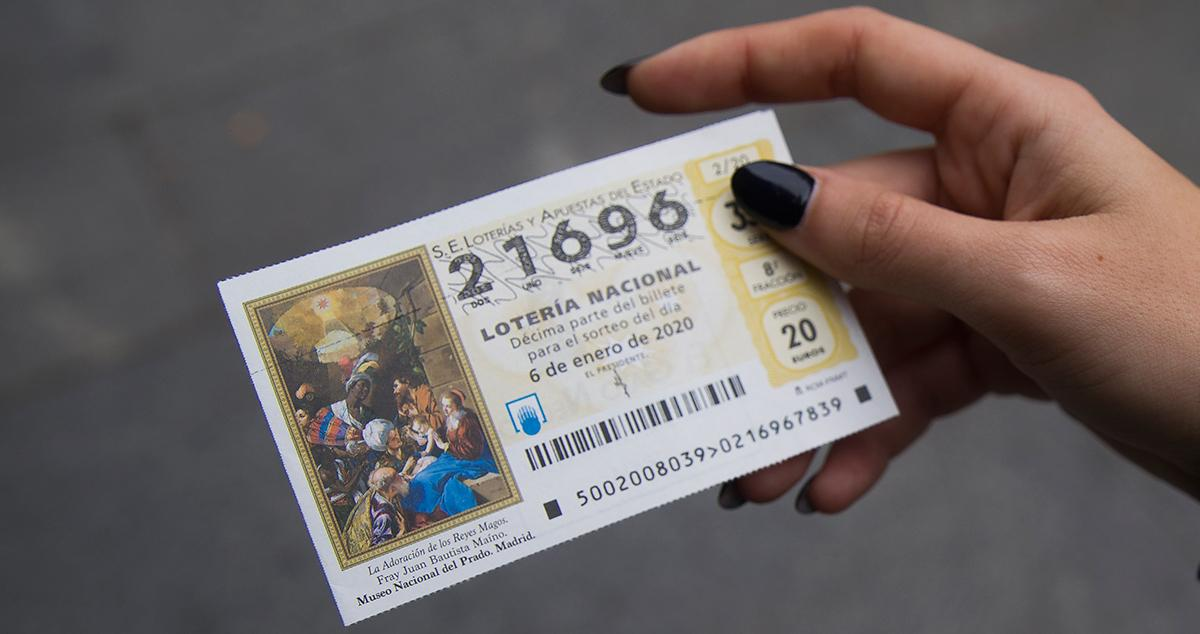
\includegraphics[width=0.4\textwidth]{figs/Fig2.jpg}
	\caption{Detecció de l’andròmina.}
	\label{f:detall}
\end{figure}

Curabitur pretium semper sem sed posuere. Quisque pre-tium ex at pellentesque ultrices. Donec dignissim urna sit amet semper sollicitudin. Sed vel vehicula metus. Praesent eleifend, lectus sit amet ornare dignissim, nibh eros vehicula dolor, at dapibus eros risus et enim. In vel porta velit, vel elementum diam. Proin at ipsum eu metus tempus euismod ac in nisl. Interdum et malesuada fames ac ante ipsum primis in faucibus. Curabitur pulvinar, dolor sit amet ultrices porttitor, odio nisl tincidunt magna, sed dapibus elit tellus vel mauris. Quisque interdum bibendum tellus, in interdum dui tincidunt vehicula. Nam laoreet ut felis id interdum. Nulla aliquet lacus eros, eu tristique risus pulvinar vel. Cras nec condimentum nulla. Nulla dapibus turpis fermentum neque pharetra, et eleifend turpis mattis. 

Integer maximus, diam eu tristique tincidunt, tellus sem sagittis urna, ac viverra nisi nibh nec lectus. Morbi mollis tincidunt ligula, in vestibulum lectus condimentum eu. Cras nec porttitor nibh. Fusce bibendum eu nunc nec eleifend. Morbi id nulla accumsan nisi suscipit tempus. Donec mollis sem enim. Praesent hendrerit dignissim tellus nec imperdiet. Proin id dapibus diam. Sed semper, ligula at iaculis dignis-sim, libero ipsum dignissim elit, at ornare ipsum risus a dolor. Phasellus vitae nibh eu purus hendrerit dapibus sit amet eget diam. Donec gravida suscipit dui, nec placerat dolor congue sit amet. Donec lobortis, justo iaculis aliquam condimen-tum, felis ligula tempor nunc, ullamcorper tincidunt ante nunc vitae sapien.

Orci varius natoque penatibus et magnis dis parturient montes, nascetur ridiculus mus. Sed eu aliquet orci. Etiam nec ultricies neque, vel semper nunc. Nullam tempus, leo at laoreet congue, ipsum tellus tempus libero, quis iaculis sapi-en lacus in sapien. Ut sapien lectus, semper eget odio in, interdum dignissim enim. Phasellus vitae purus gravida, rutrum ante vel, vestibulum mauris. In eget diam convallis, pellentesque tortor sit amet, consectetur augue. Vestibulum sed rhoncus augue. Aenean consectetur ligula vitae sapien molestie. 


\section{Conclusions}

Aliquam erat volutpat. Pellentesque habitant morbi tristi-que senectus et netus et malesuada fames ac turpis egestas. Donec ut sapien nec turpis placerat maximus. Quisque port-titor nulla ex, vel finibus nisi commodo in. Vivamus fringilla diam eget est egestas, id hendrerit leo tincidunt. Mauris tin-cidunt iaculis ornare. Curabitur pulvinar, dolor amet ultrices porttitor, odio nisl tincidunt magna, sed dapibus elit tellus vel mauris. Proin faucibus scelerisque orci vitae aliquet. Nulla ullamcorper tincidunt nisl, sit amet mollis mi pretium sit amet. Fusce sagittis vehicula nibh, ut pulvinar magna ves-tibulum eget. Praesent vulputate accumsan eros sed portti-tor. 

Quisque consectetur justo a mi porta, id varius nisi posue-re. Morbi tristique orci nec dolor aliquet venenatis. Integer malesuada tincidunt dignissim. Cras lobortis metus tristique erat placerat, nec rutrum justo pretium. Integer faucibus aliquet commodo. Integer non quam nec lectus. Sed in leo rhoncus, gravida elit vel, tristique quam. Nullam auctor mi in tortor mollis ullamcorper. 

Nunc dictum ipsum quis egestas scelerisque. Vestibulum rutrum tempor posuere. Praesent varius libero odio, ac bibe-ndum arcu tempus quis. Pellentesque habitant morbi tristi-que senectus et netus et malesuada fames ac turpis egestas. Sed eget ex risus. Integer metus velit, viverra ac fringilla sit amet, laoreet eget lacus. Nulla rutrum mollis elit et maximus. Nulla sed aliquet elit. Sed libero justo, porta ut vulputate eget, suscipit faucibus sem. Sed at quam ut justo vestibulum vehicula non sed ligula. 

Nulla facilisi. Curabitur pulvinar, dolor amet ultrices porttitor, odio nisl tincidunt magna, cras lobortis metus tristique erat placerat, sed dapibus elit tellus vel mauris. Phasellus vitae purus gravida, rutrum ante vel, vestibulum mauris. 


\begin{thebibliography}{9}
\bibitem{latex} \LaTeX. (21 d'Abril de 2021). A Wikibooks. http://en.wikibooks.org/wiki/LaTeX
\bibitem{Russakovskyet2015} O. Russakovskyet al., ``ImageNet large scale visual recognition challenge,'' Int. J. Comput. Vis., vol. 115, no. 3, pp. 211–252, 2015.
\bibitem{Krizhevsky2012} A. Krizhevsky, I. Sutskever, and G. E. Hinton, ``ImageNet classifica-tionwith deep convolutional neural networks,'' inProc. Int. Conf. Neural Inf.Process. Syst., 2012, pp. 1097–1105.
\bibitem{Simonyan2014} K. Simonyan and A. Zisserman, ``Very deep convolutional networks forlarge-scale image recognition,'' inProc. Int. Conf. Learn. Repre-sentations, 2014.
\bibitem{Szegedyet2015} C. Szegedyet al., ``Going deeper with convolutions,'' inProc. IEEE Conf.Comput. Vis. Pattern Recognit., Jun. 2015, pp. 1–9.
\end{thebibliography}
\end{document}

